\chapter{Model training}
\section{Training framework}
For model training, we used PyTorch as our training framework due to its flexibility compared to other machine learning libraries such as TensorFlow. Regarding the code implementation of these models in PyTorch, the UNet architecture was implemented by us following the scheme illustrated in the Figure 2.2. Whereas other architectures, such as UNet++ and Attention UNet, were obtained from publicly available GitHub repositories where corresponding implementations had been published [24, 25]. As for the DeepLabV3 model, it is included in the torchvision library (an extension of PyTorch). We therefore loaded it directly in PyTorch with a ResNet backbone pretrained on the ImageNet dataset. Since the default DeepLabV3 configuration is designed for multiclass segmentation, we applied a minor modification to its final layer by adding a sigmoid activation function, ensuring the output values are constrained between 0 and 1.\\


\section{Grid search}
Before training the model, a grid search has been carried out using the validation set for each architecture in order to determine the optimal hyperparameters. However, due to the limited time for implementation and computational limitations, we restricted the search to only three hyperparameters: learning rate (tested values: 1e‑3, 5e‑4 and 1e‑4), batch size (tested values: 4, 8 and 16), and the number of filters (several combinations were evaluated on the UNet architecture). To further reduce memory consumption, all training images were resized to 512 x 512 pixels. The optimizer used during the search was Adam [23], and the loss function was BCE (binary cross entropy), MSE (mean square error) was also tested but no greater results have been observed. The optimal hyperparameters obtained during the grid search are shown in the table below:
\begin{table}[H]
\centering
\begin{tabular}{|c|l|l|}
\hline
\textbf{Model}            & \multicolumn{1}{c|}{\textbf{Learning rate}} & \multicolumn{1}{c|}{\textbf{Batch size}} \\ \hline
\textbf{UNet}           & 0.001                                       & 4                                        \\ \hline
\textbf{UNet++}         & 0.001                                       & 4                                        \\ \hline
\textbf{Attention UNet} & 0.0001                                      & 4                                        \\ \hline
\textbf{DeeplabV3+}     & 0.0001                                      & 4                                        \\ \hline
\end{tabular}
\caption{Optimal hyperparameters}
\label{tab:my-table}
\end{table}


% \begin{figure}[H]
%  \centering
%  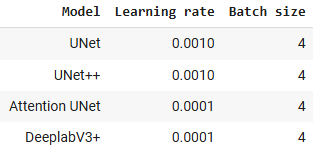
\includegraphics[scale=0.9]{IMAGENES/gridsearch.png}
%  \captionsetup{font=large}
%  \caption {Optimal hyperparameters}
% \end{figure}

\section{Preliminary training and architecture comparison}
Once the optimal hyperparameters were determined, we performed a reduced model training for each architecture using its corresponding optimal hyperparameters. As in the grid search phase, this training was performed on LoveDA Dataset only. The purpose of this stage was to determine which architecture best fits our segmentation task, and the most promising architecture identified here will later be used to perform a more complete model training, incorporating the full dataset, image augmentation, L2 regularization, etc.\\

Model evaluation was based on metrics derived from the confusion matrix. Specifically, for each architecture, predictions were generated on the validation dataset in the form of binary masks (matrices containing values of 0 and 1). These predicted masks were then compared with the corresponding ground-truth masks to construct the confusion matrix.\\

\begin{figure}[H]
 \centering
 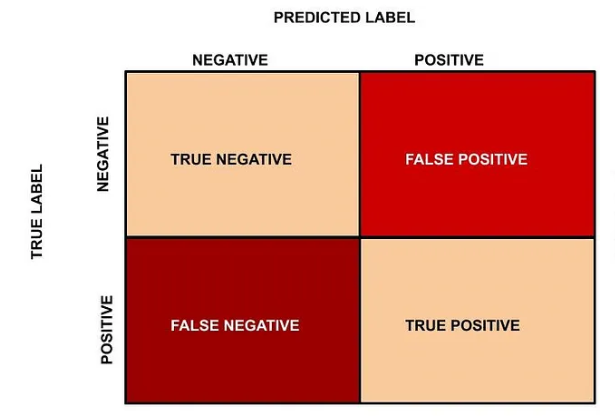
\includegraphics[scale=0.8]{IMAGENES/IMG16-CM.PNG}
 \captionsetup{font=large}
 \caption {Confusion matrix (In our case, we can consider negative as 0 and positive as 1)}
\end{figure}

The confusion matrix provides information about the number of correctly and incorrectly classified pixels, from which several metrics can be calculated to evaluate model performance. In this project, we considered three evaluation metrics:\\
\begin{itemize}
    \item \textbf{Accuracy}: This metric measures the proportion of correctly classified pixels relative to the total number of pixels, and can be determined using the following equation.\\
    \begin{equation}
    \text{Accuracy} = \frac{TP + TN}{TP + TN + FP + FN}
    \end{equation}
    \item \textbf{F1 score}: The F1 score is the harmonic mean of precision and recall, balancing false positives and false negatives, and can be determined in the following way.
    \begin{equation}
        F_{1} = \frac{2 \cdot TP}{2 \cdot TP + FP + FN}
    \end{equation}
    \item \textbf{Area under the ROC curve (AUC)}:  Since each architecture includes a final sigmoid activation layer, the raw model outputs are probability maps with values between 0 and 1 rather than strictly binary masks. To convert these into binary predictions, a threshold must be applied (for the accuracy and f1 score, we have considered a threshold of 0.5). The receiver operating characteristic (ROC) curve evaluates model performance for different threshold values, plotting the true positive rate against the false positive rate. The area under the ROC curve (AUC) summarizes this performance: a larger AUC indicates that the model is more robust and less sensitive to threshold variation. 
\end{itemize}

\section{Architecture selection}
The results obtained from the model comparison are shown in the figure below: 
\begin{table}[H]

\begin{tabular}{|c|l|l|l|l|l|}
\hline
\textbf{Architecture}            & \multicolumn{1}{c|}{\textbf{Num. of parameters}} & \multicolumn{1}{c|}{\textbf{Inference time/image (s)}} & \multicolumn{1}{c|}{\textbf{Accuracy}} & \multicolumn{1}{c|}{\textbf{F1 score}} & \multicolumn{1}{c|}{\textbf{AUC}} \\ \hline
\textbf{UNet}           & 9M                                               & 0.0047                                                 & 0.801                                  & 0.827                                  & 0.838                             \\ \hline
\textbf{UNet++}         & 31M                                              & 0.0145                                                 & 0.659                                & 0.762                                  & 0.795                             \\ \hline
\textbf{Attention UNet} & 8M                                               & 0.0063                                                 & 0.866                                  & 0.878                                  & 0.843                             \\ \hline
\textbf{DeeplabV3+}     & 41M                                              & 0.0116                                                 & 0.895                                  & 0.907                                  & 0.879                             \\ \hline
\end{tabular}
\caption{Model comparison. The table includes the number of parameters, inference time, accuracy, f1 score and AUC for each architecture.}
\label{tab:my-table}
\end{table}

%  \begin{figure}[H]
%  \centering
%  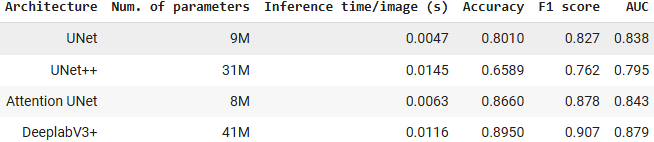
\includegraphics[scale=0.9]{IMAGENES/comparison.png}
%  \captionsetup{font=large}
%  \caption {Model comparison. The table includes the number of parameters, inference time, accuracy, f1 score and AUC for each architecture.}
% \end{figure}

As shown, DeepLabv3+ outperforms the other model architectures in all evaluation metrics, with an only drawback which is its relatively longer inference time. However, this limitation is outweighed by its high accuracy. Also, the high AUC score indicates that the architecture is robust to variations in the decision threshold. Thus, we considered that the DeepLabv3+ was the most suitable architecture for our segmentation task, and the complete training and inference in the following section were all conducted using this model architecture.\\


\section{Complete model training}
Once the best model architecture was selected, we proceeded to perform a more comprehensive training using the complete Jordan Forest and LoveDA datasets. During model training, 3 image augmentations were applied in order to enhance the model’s generalization ability. These augmentations include:\\



\begin{itemize}
    \item \textbf{Random resize crop}: A random portion of the input image is selected and resized to 512 x 512 pixels. This aims to help the model to handle images of varying resolutions. Although the training datasets contain high-resolution images, we also want to raise the model performance on lower-resolution inputs.
    \item \textbf{Color jitter}: Random modifications are applied to brightness, contrast, saturation, and hue. This helps the model adapt to variations caused by different camera setups and seasonal changes. 
    \item \textbf{Vertical and horizontal flip}: The image is randomly flipped along the horizontal or vertical axis. This augmentation may not always increase the model performance, but it is a free approach to increase training data size. 
\end{itemize}

Additionally, a L2 regularization has also been applied to prevent overfitting. This regularization introduces an additional term into the loss function that penalizes large weight values, which helps to reduce the model's complexity.

Another modification in the training process was that, instead of selecting only the best model epoch, we retained all epochs where the models achieve both an Accuracy and an F1 score greater than 0.9 on the training set (Jordan Forests and LoveDA) and greater than 0.8 on the validation set (Cantabria). We adopted a lower threshold for performance on the Cantabria set because it was not used during training, thus it would be more difficult for the model to achieve high performance on it.

The complete training resulted in 12 models, 6 were trained on the Jordan Forests Dataset and 6 on the LoveDA Dataset. We chosed to trained on these datasets separately because of the imbalance in the number of training samples and the difference in the image resolution. As mentioned earlier, the Jordan Forests Dataset contains more than 4000 images with a resolution of 2160 x 3840 pixels, whereas the Loveda Dataset has only about 300 images with a resolution of 1024 x 1024 pixels. Althogh both datasets will undergo the same preprocessing steps, which would resize all images to 512 x 512 pixels, but the imbalance in the number of samples would cause the model to be dominated and biased by the larger dataset. In order to handle this imbalance, we attempted oversampling the smaller dataset by duplicating samples and applying random augmentations. However, this has eventually led to a downgrade in model performance. Therefore, we decided to train the models separately on each dataset.\\

